\documentclass[10pt,a4paper,mathserif]{beamer}
\usepackage[utf8x]{inputenc}
\usepackage{ucs}
\usepackage[english,russian]{babel}
\usepackage{amsmath}
\usepackage{amsfonts}
\usepackage{amssymb}
\usepackage{mathtext}
\usepackage{graphicx}
\usepackage{enumerate}
\usepackage{multirow}
\usepackage{caption}
\usepackage{subcaption}

\usetheme {Madrid}
\usecolortheme [RGB={85, 107, 47}]{structure}

\title{Производственная практика: технологическая (проектно-технологическая) практика}
\subtitle{Разработка игры Pac-man на языке программирования Python}
\author{Давыдов М.А.}
\institute{группа 5.205-1}
\date{\today}

\begin{document}

\begin{frame}
\maketitle
\end{frame}

\begin{frame}{Актуальность}
    \begin{block}{}
    По сей день аркадные игры популярны среди игроков различных возрастов, так как они позволяют скоротать время в поездке или, например, на лекции, на скучном собеседовании.
    \end{block}

    \begin{block}{}
    Разработка игры в жанре <<Аркада>> позволяет сформировать представление о самом её <<скелете>>, о её графической составляющей, о правильном построении алгоритмов.
    \end{block}

    \begin{block}{}
    Разработка кроссплатформенной программы на языке программирования Python может послужить хорошим стимулом как для более глубокого изучения программирования, так и для понимания сборки программы под различные платформы.
    \end{block}
\end{frame}

\begin{frame}{Цель и задачи}
    \begin{block}{Цель:}
        \small{Создать кроссплатформенную игру Pac-man с использованием языка программирования Python3 и библиотеки PySDL2.}
    \end{block}

    \begin{block}{Задачи:}
        \begin{itemize}
            \item \small{Изучить графическую библиотеку PySDL2.}
            \item \small{Изучить алгоритмы игры Pac-man.}
            \item \small{Научиться выставлять собственную частоту кадров игровой области.}
        	\item \small{Разобраться во взаимодействии компьютерной графики с аппаратным или программным обеспечением.}
        	\item \small{Изучить сборку программы на языке Python под ОС Microsoft Windows и GNU/Linux.}
        	\item \small{Изучить принцип ООП в Python.}
        	\item \small{Закрепить навыки в работе с системой компьютерной вёрстки \TeX и его расширения \XeTeX.}
        \end{itemize}
    \end{block}

\end{frame}

\begin{frame}{Обзор инструментария для создания компьютерной игры}
    \begin{block}{Графическая библиотека}
            \textbf{PySDL2} --- это чистая оболочка Python для библиотек \textit{SDL2, SDL2\_mixer, SDL2\_image, SDL2\_ttf и SDL2\_gfx}. 
    \end{block}

    \begin{block}{Инструментарий}
    \begin{itemize}
        \item Для написания отчёта с помощью системы компьютерной верстки в \TeX{} была использована IDE TexStudio, а также дистрибутив Tex Live.
        \item Для написания кода программы была использована IDE Microsoft Visual Studio Code.
        \item Для работы с текстурами был использован графический редактор Adobe Photoshop 2023.
    \end{itemize}
    \end{block}
\end{frame}

\begin{frame}{Обзор инструментария для создания компьютерной игры}
    \begin{block}{Игра Pac-Man}
        \textbf{Pac-Man} --- аркадная видеоигра, разработанная японской компанией Namco и вышедшая в 1980 году.
    \end{block}

    \begin{block}{Правила игры}
        Экран игры представляет собой лабиринт, коридоры которого заполнены точками. Задача игрока --- управляя Пакманом, съесть все точки в лабиринте, избегая встречи с привидениями, которые гоняются за героем.
    \end{block}
\end{frame}

\begin{frame}{}
    \vspace{-0.5cm}\begin{figure}[H]
      \centering
      \hspace{-0.5cm}
\includegraphics[width=1\textwidth]{src/1.png}
    \end{figure}
\end{frame}

\begin{frame}{Код программы}
    \begin{figure}
    \centering
    \begin{subfigure}{.5\textwidth}
      \centering
      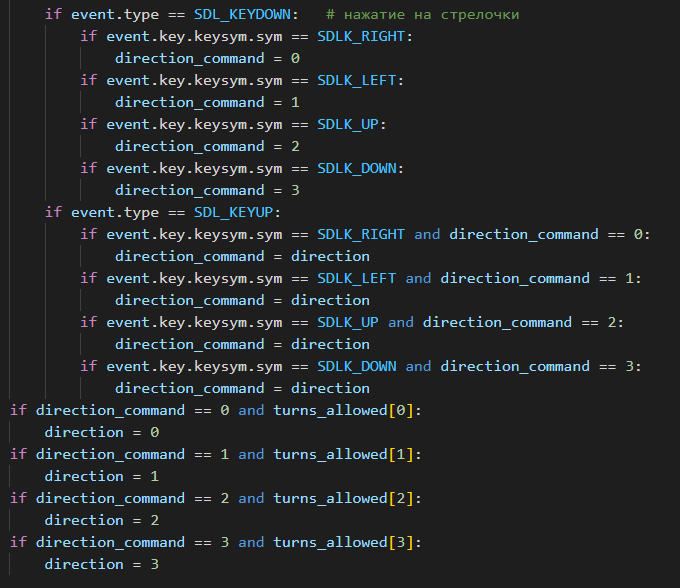
\includegraphics[width=.98\linewidth]{src/code1.png}
      \caption{Обработка нажатий.}
    \end{subfigure}%
    \begin{subfigure}{.5\textwidth}
      \centering
      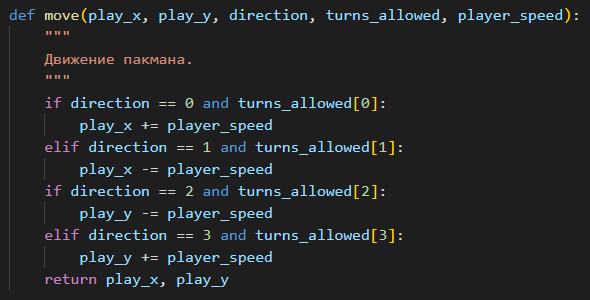
\includegraphics[width=.98\linewidth]{src/code2.png}
      \caption{Функция движения пакмана.}
    \end{subfigure}
    \end{figure}
\end{frame}

\begin{frame}{Тестирование игры}
    \begin{figure}
    \centering
    \begin{subfigure}{.5\textwidth}
      \centering
      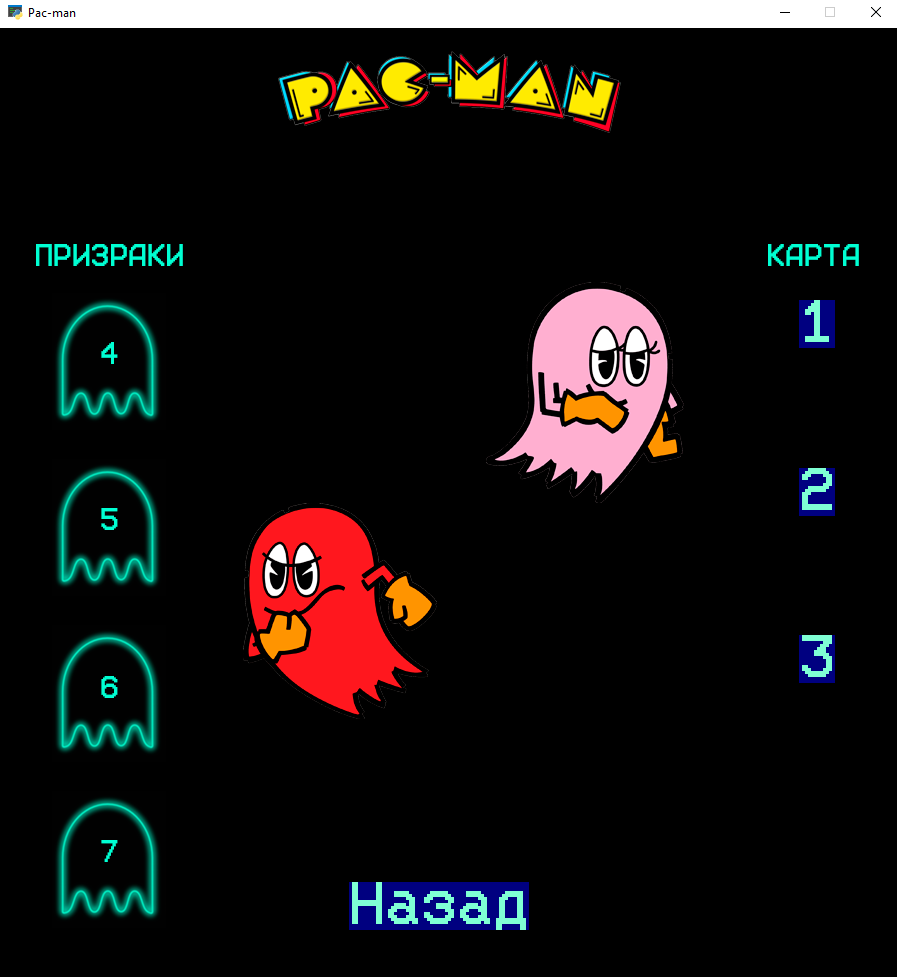
\includegraphics[width=.8\linewidth]{src/3.png}
      \caption{Экран выбора.}
    \end{subfigure}%
    \begin{subfigure}{.5\textwidth}
      \centering
      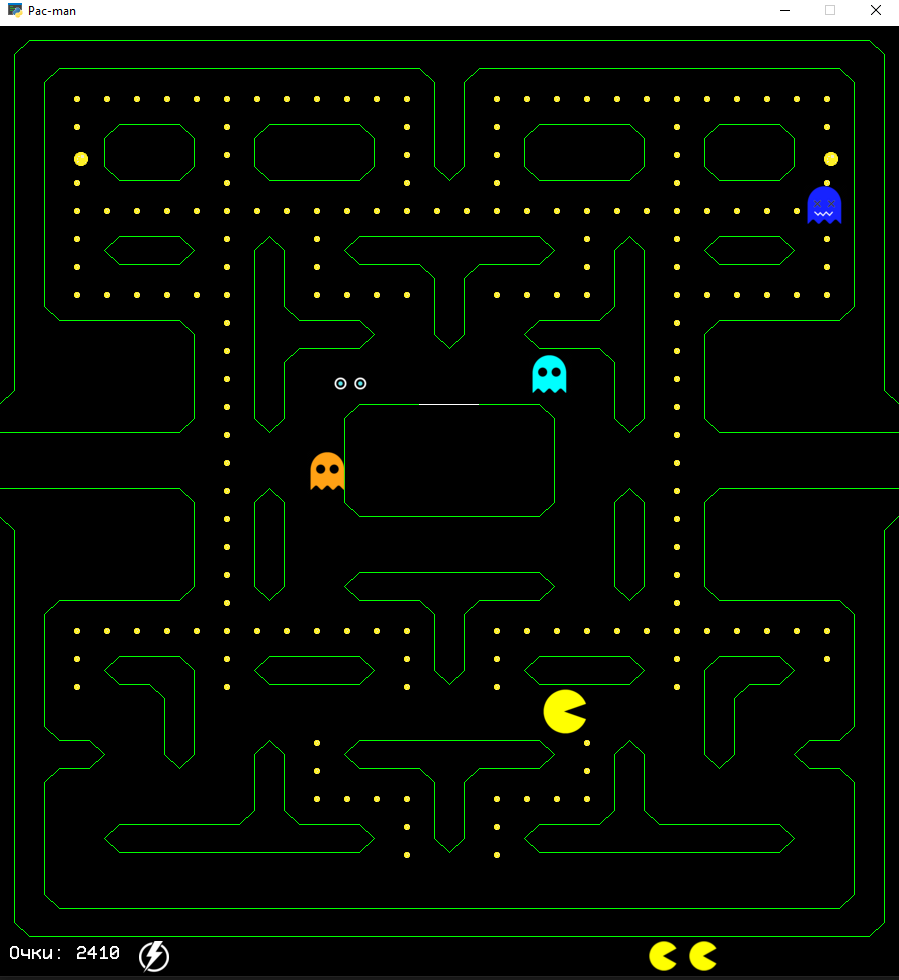
\includegraphics[width=.8\linewidth]{src/5.png}
      \caption{Игровой процесс.}
    \end{subfigure}
    \end{figure}
\end{frame}

\begin{frame}{Заключение}
    \begin{block}{}
        В ходе выполнения лабораторной работы была создана кроссплатформенная программа с использованием языка программирования Python3 и библиотеки PySDL2.
    \end{block}

    \begin{block}{}
        Кнопки срабатывают при нажатии на них, при этом меняется экран. Выбор карты и количества призраков успешно выполняется. Пакман управляется стрелками, призраки гоняются за ним. Все взаимодействия между пакманом, точками, призраками и лабиринтом успешно отрабатываются.
    \end{block}

    \begin{block}{}
        Разработка программы и отчёта производилась с использованием системы контроля версий Git, а именно с помощью онлайн-хранилища GitHub.
    \end{block}
\end{frame}

\end{document}
